\documentclass{sig-semester}

\pdfpageheight=11in
\pdfpagewidth=8.5in

\usepackage{latexsym}
\usepackage{amsmath}
\usepackage{amssymb}
\usepackage{color}
\usepackage{enumerate}
\usepackage{amssymb}
\usepackage{xspace}
\usepackage{graphicx}
\usepackage{epstopdf}

% These are from candidacy edic.tex
\graphicspath{{./graphics/}}
\DeclareGraphicsExtensions{.pdf,.jpeg,.png}

% Legacy from Christoph's paper:
% \DeclareGraphicsRule{.tif}{png}{.png}{`convert #1 `dirname #1`/`basename #1 .tif`.png}

% When converting eps to pdf, suffix is added to filename. 
% Recommended not to be empty string by http://www.tex.ac.uk/tex-archive/macros/latex/contrib/oberdiek/epstopdf.pdf : page 4, suffix paragraph.
\epstopdfsetup{suffix=-generated}

\newtheorem{theorem}{Theorem}[section]
\newtheorem{proposition}[theorem]{Proposition}
\newtheorem{example}[theorem]{Example}
\newtheorem{remark}[theorem]{Remark}
\newtheorem{todo}[theorem]{ToDo}
\newtheorem{algorithm}[theorem]{Algorithm}
\newtheorem{metatheorem}{Metatheorem}[section]
\newtheorem{definition}[theorem]{Definition}
\newtheorem{property}[theorem]{Property}
\newtheorem{corollary}[theorem]{Corollary}
% \newtheorem{lemma}[theorem]{Lemma}
\newtheorem{conjecture}[theorem]{Conjecture}
\newtheorem{proviso}[theorem]{Proviso}


\title{DBToaster generated program analysis}


%\numberofauthors{1}
\author{\alignauthor Aleksandar Vitorovic \\[1ex]
\affaddr{Dept.\ of Computer Science} \\
\affaddr{EPFL} \\
\affaddr{aleksandar.vitorovic@epfl.ch}
}

\def\SQL{SQL\xspace}
\def\OLAP{OLAP\xspace}
\def\OLTP{OLTP\xspace}
\def\M3{M3\xspace}
\def\EXORD{actual OLAP update execution order\xspace}

\hyphenation{cau-sality lo-gically}

\begin{document}
\maketitle

\abstract{The goal of this paper is to analyze typical M3 programs generated by DBToaster and to find a way to efficiently execute them in parallel.\\
}

\keywords{Data-parallelism, map partitioning, trigger partitioning}

\section{Introduction}
\vspace{2mm}
In this paper M3 programs characteristics are studied in order to find an efficient way to execute them in a parallel environment. Typical patterns in the code are described, as well as their connection to map and trigger partitioning. By putting all the ideas together, it may be possible to further simplify our system design, and even avoid using corrective updates at all.

All the term used here are defined in semesterPaper.pdf. For example, trigger instantiation is the same as update event or update. If not explicitly stated otherwise, all the maps are stored on separate nodes.

For each sql query transformed to M3 program, the following are presented: original query, generated M3 program, and a list of cycles breaking atomicity on trigger level. Furthermore, for each sql query, map and trigger partitioning are explained in context of alleviating these atomicity cycles. All the conclusions from the programs are put in the last section of the paper.

\section{Queries}
\vspace{2mm}

\subsection{rs.sql}
\textbf{Query.} This query is actually:
\begin{verbatim}
SELECT SUM(A*C) FROM R,S WHERE R.B = S.B.
\end{verbatim}

\textbf{M3 program.} The generated M3 is:
\begin{verbatim}
    ON +S[A; B] 
S.1 m1 += m2[A] * B
S.2 m3[A] += B

    ON +R[A; B] 
R.1 m1 += A * m3[B]
R.2 m2[B] += A
\end{verbatim}
This program differs from the original M3 program in the way that naming scheme is simplified and long names for variables and constants are avoided. The A and B variables in the M3 program may not refer to A and B from the query. Similar simplification of M3 programs are applied to all the queries in the rest of this paper.

The triggers for deletion are not shown, since they are symmetric to the insert triggers. The only difference is multiplying the terms with -1.

\textbf{Conditions for violating atomicity.} In order to preserve atomicity, all the affected maps have to have the same value as update events were executed in some serial order. For this particular query, atomicity is violated if all the following conditions are met:
\begin{enumerate}[(1)]
 \item An S trigger and an R trigger arrives from multiple input points at the appropriate same time,
 \item Statements are executed in an order such that neither event sees the effect of the other one (``too-little`` data), or both of them sees the effect of the other one (``too-much`` data),
 \item Update event parameters equality: S.A = R.B.
\end{enumerate}

The parameters from different triggers which participate in the parameters equality relations are denoted as \textit{conflict parameters}.

As we can see, the third condition for breaking atomicity is essentially a WHERE clause from the SQL query. This is generally true if there are no loop variables in a M3 program.

When atomicity is violated in M3 programs, it is formed out of two statements from two update events from different triggers. This structure will be called cycle: the lhs from a statement from one trigger is a rhs from a statement from another trigger, and a rhs from the first trigger is the lhs from the second trigger. The lhs and rhs of both the triggers refers to different statements inside trigger, so statements themselves never form a cycle. In this query, a cycle is formed between S and R update event, if S.A = R.B. Both statement and trigger graph of the query are presented in Figure~\ref{fig:rs}.

\begin{figure}[!t]
\centering
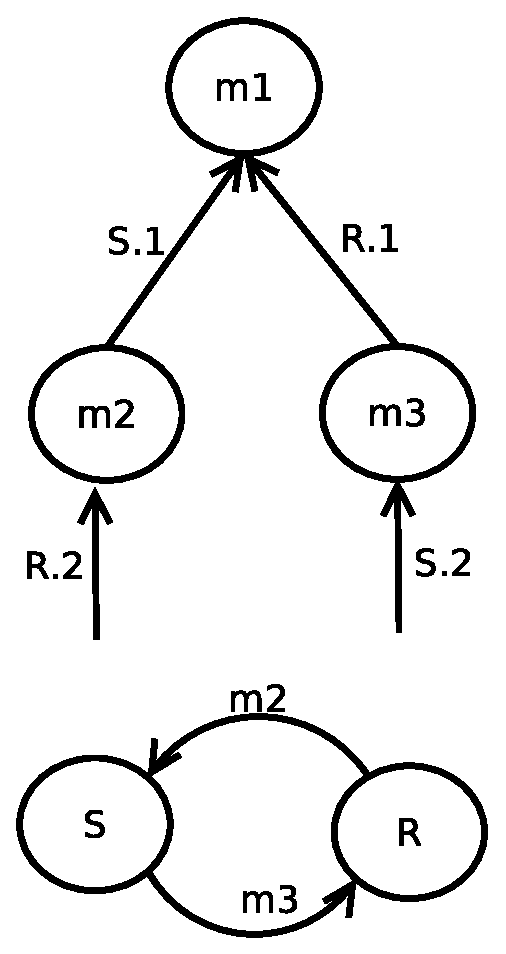
\includegraphics[width=1in]{rs.eps}
\vspace{-3mm}
\caption{Statement and trigger graph for rs.sql.}
\label{fig:rs}
\vspace{-2mm}
\end{figure}

In the ``too-little`` data scenario, the statement R.1 does not see the new value of m3 from S.2, and the statement S.1 does not see the new value of m2 from R.2. In other words, the node containing m2 sees the S, R order, while the node containing m3 sees the R, S order. This is possible due to the fact that update events arrive from different input points, and we assumed that network guarantees only pair-wise in-order delivery. The following schedules meet these conditions:
\begin{verbatim}
 1) R.1 S.1 R.2 S.2
 2) R.1 S.1 S.2 R.2
 3) R.1 S.2 S.1 R.2
 4) S.1 R.1 R.2 S.2
 5) S.1 R.1 S.2 R.2
 6) S.1 R.2 R.1 S.2
\end{verbatim}
These schedules depicts possible wall clock time of execution statements. Since different statements inside trigger relate to different maps, they may arrive out-of-order.

This situation can be avoided efficiently by the corrective update mechanism. After receiving an S update event, the node containing m2 cannot block waiting for R event to arrive, since it cannot distinguish between non-existing update events and unpredictable latency in the network.

In the ''too-much`` data scenario, the statement R.1 sees the new value of m3 from S.2, and the statement S.1 sees the new value of m2 from R.2. In other words, the node containing m2 sees the R, S order, while the node containing m3 sees the S, R order. Again, this is a consequence of using multiple input points. The following schedules meet these conditions:
\begin{verbatim}
 1) S.2 R.2 S.1 R.1
 2) S.2 R.2 R.1 S.1
 3) S.2 R.1 R.2 S.1
 4) R.2 S.2 S.1 R.1
 5) R.2 S.2 R.1 S.1
 6) R.2 S.1 S.2 R.1
\end{verbatim}
As before, the schedules depicts possible wall clock time of statements' execution. Again, since different statements inside trigger relate to different maps, they may arrive out-of-order.

There are mechanisms to avoid this situation by filtering on the sending side. The sender will compare the order it observes with a canonical order and send the appropriate (old) version of a map. More details can be found in looseCumulus.pdf file.

In terms of R/W dependencies, there is always a W-R dependency and a R-W dependency between update events forming a cycle. In M3 programs generated by DBToaster, these dependencies only appear as part of a cycle. The W-W dependencies are transformed into multiple W/R or R/W dependencies upon arrival of an update event reading from particular map. Thus, if our system handle atomicity violation correctly, all the dependencies will be preserved as well.

We can put all the necessary information about the cycle in a short form:
\begin{verbatim}
Condition: 
S.A = R.B (no-loop)

M3 program, dependencies:
    ON +S[A; B] 
S.1 m1 += m2[A] * B
S.2 m3[A] += B, S->R
    ON +R[A; B] 
R.1 m1 += A * m3[B]
R.2 m2[B] += A, R->S
\end{verbatim}
The X->Y sign next to a statement represents that the map on the lhs of the statement in X trigger is used on the rhs of Y trigger.

In this paper, as a major contribution, we propose two different solution for preserving atomicity without the corrective update mechanism and the filtering approach: the trigger and map partitioning. The former is based on a source ordering principle, since all the events that possibly can cause atomicity violations are ordered through a single input point in the system. The latter is based on a destination ordering principle, since all the events that possibly can cause atomicity violations are ordered through a single node, thus avoiding different views of the system from different maps. In addition, when any of the two approaches, only the last version of a map has to be preserved.

\textbf{The trigger partitioning solution.} The solution is to partition update events on their conflict parameter (S on A and R on B). All the update events with the same conflict parameter's range have to be processed through a single input point.

\textbf{The map partitioning solution.} The solution is to partition maps in such a way so that the nodes containing m2 and m3 do not see update events in different order. The same ranges of m2 and m3 maps have to be stored on the same physical node.

Both solutions are possible due to non-existence of loop variables in the M3 program.

\subsection{rsgb.sql}
\textbf{Query.} This query is actually:
\begin{verbatim}
SELECT C,SUM(A) FROM R,S WHERE R.B=S.B GROUP BY C.
\end{verbatim}

\newpage
\textbf{M3 program.} A simplification of generated M3 paired with a cycle condition is presented here:
\begin{verbatim}
ON +S[A; B]: 
 m1[B] += m2[A]
 m3[A; B] += 1

ON +R[A; B]:
 m1[C] += A * m3[B; C]
 m2[B] += A

Condition: S.(A,B) = R.(B,C) and R.B = S.A
equivalent to: S.A = R.B and S.B = R.C
\end{verbatim}

As with rs.sql, enough condition for preserving atomicity is S.A = R.B, which can be preserved in the same way as in rs.sql.

\subsection{sum.sql}
\textbf{Query.} This query is actually:
\begin{verbatim}
SELECT sum(A) FROM R.
\end{verbatim}

\textbf{M3 program.} A simplification of generated M3 is presented here:
\begin{verbatim}
ON +R[A; B]
m1 += A
\end{verbatim}

There is no possibility for creation of cycles in this example.

\subsection{sumgb.sql}
\textbf{Query.} This query is actually:
\begin{verbatim}
SELECT B, sum(A) FROM R group by B.
\end{verbatim}

\textbf{M3 program.} A simplification of generated M3 is presented here:
\begin{verbatim}
ON +R[A; B]:
m1[B] += A
\end{verbatim}

There is no possibility for creation of cycles in this example.

\subsection{rst.sql}
\textbf{Query.} This query is actually:
\begin{verbatim}
SELECT SUM(A*D) FROM R,S,T 
WHERE R.B = S.B AND S.C = T.C.
\end{verbatim}

\textbf{M3 program.} A simplification of generated M3 paired with dependencies is presented here:
\begin{verbatim}
    ON +R[A; B]
R.1 m1 += A * m4[B]
R.2 m2[C] += A * m5[B; C], R->T
R.3 m3[B] += A,            R->S

    ON +S[A; B] 
S.1 m1 += m3[A] * m6[B]
S.2 m2[B] += m3[A],        S->T
S.3 m4[A] += m6[B],        S->R
S.4 m5[A; B] += 1,         S->R; S->T

    ON +T[A; B]
T.1 m1+= m2[A] * B
T.2 m4[C] += B * m5[C; A], T->R
T.3 m6[A] += B,            T->S
\end{verbatim}

Trigger S has one more statement and no loop variables since it appears in two join conditions.

Here we can create cycles from only two triggers (we will denote them as 2-cycles), and cycles out of all three triggers (we will denote them as 3-cycles). The 2-cycles are of the same form as the only cycle in the rs.sql.

Now, we will enumerate all the 2-cycles for rst.sql:
\begin{verbatim}
 (1) R->T: R.2 T.1, m2
     T->R: T.2 R.1, m4
     Condition: R.C = T.A and T.C = R.B (loop)

 (2) R->S: R.3 S.1, m3
     S->R: S.3 R.1, m4
 (3) R->S: R.3 S.2, m3
     S->R: S.3 R.1, m4
     Condition: R.B = S.A and S.A = R.B
     equivalent to: R.B = S.A (non-loop)

 (4) R->S: R.3 S.1, m3
     S->R: S.4 R.2, m5
 (5) R->S: R.3 S.2, m3
     S->R: S.4 R.2, m5
     Condition: R.B = S.A and S.(A,B) = R.(B,C)
     equivalent to: R.B = S.A and S.B = R.C (loop)

 (6) S->T: S.2 T.1, m2
     T->S: T.3 S.1, m6
 (7) S->T: S.2 T.1, m2
     T->S: T.3 S.3, m6
     Condition: S.B = T.A and T.A = S.B
     equivalent to: S.B = T.A (non-loop)

 (8) S->T: S.4 T.2, m5
     T->S: T.3 S.1, m6
 (9) S->T: S.4 T.2, m5
     T->S: T.3 S.3, m6
     Condition: S.(A,B) = T.(C, A) and T.A = S.B
     equivalent to: S.A = T.C and S.B = T.A (loop)
\end{verbatim}

There are three conditions with loops and two without loops. All the conditions without loops are symmetric. All the maps except m1 are shown in exactly two conditions. Except the first cycle, all the other can be avoided by serializing update events such that R.B = S.A and S.B = T.A. In addition, by preserving non-loop part of the condition for (4),(5),(8),(9), we forbidden data dependencies in both directions. All update events that are data dependent are ordered by map or trigger partitioning, so computation is entirely data-parallel.

Another important property of M3 programs is that a map always use exactly the same parameters all around a trigger, so the same conditions are necessary for each cycle created out of the two same maps (i.e (4) and (5), (6) and (7), etc.).

\textbf{Condition loops.} There are two different types of loops in conditions. First one is in the cycle (5) and the cycle can be broken by avoiding non-loop condition R.B = S.A. Second one is in the cycle (1), and it contains loops in all condition terms. We will denote such loop as hard-loops.

The hard-loops are harder to partition. In the cycle (1), trigger partitioning solution imply that all R and T triggers are processed through the same input point, while map partitioning implies that all the m2 and m4 maps have to be put on the the node. It is interesting to note that hard-loop occurs only between tables not adjacent in the WHERE clause (sharing the same variables in joins in Cumulus algebra). Loop unrolling can also be done in runtime, causing some overhead, but further research is necessary on this topic.

Now we will show that all 3-cycles are avoided if 2-cycles are avoided. In order to have 3-cycle either S->T or T->S has to exist, but this is not possible since the S.B = T.A situations are avoided even for 2-cycles. It can be inferred that all the higher-level cycles are avoided if 2-cycles are avoided.

We will present several solutions:
\begin{enumerate}
\item The easiest solution is to process only one trigger type at the time, since there is no dependencies within trigger except Write-Write (a map is either on the lhs or on the rhs all over the trigger).
\item Process R and T simultaneously from multiple input points (even more than 2) by putting m2 and m4 on a single node, while S must be done alone in the system. Or R and S (S and T) can be done together by trigger partitioning presented for rs.sql, thus executing T (R) alone in the system. In TPCH benchmarks we can prioritize some tables which are more frequently updated. In most cases, only few relations are updated (such as CUSTOMER, LINEITEM), while the others (such as NATION, etc.) are rarely updated.

When update events from 2 triggers are processed at the same time, avoiding the conditions from WHERE clause referring to join between two relevant tables is enough for eluding 2-cycles. This is also shown on rs2joint.sql, where there are two conditions for join between R and S: R.A=S.A AND R.B=S.B.

\item An optimization of the previous approach is to keep track of currently processing trigger parameters, and let S in the system only if there are no conflicts. This is not scalable, since input points have to communicate with nodes and among themselves about completed update events.
\item Update events R and T can be processed on arbitrary input points, as long as m2 and m4 are on a single node and S is sent from two input points. For example, if R(1,4) is sent thought IP1 and T(2,9) is sent through IP2, then S(4,2) is sent through both switches.

We will prove that this approach is not working. Due to our-of-order execution, it is entirely possible that the node containing m5 first see S from the second input point before R update event from the first input point, and the node containing m3 sees R before any S update event. Thus, different nodes see a conflicting order, thus breaking the atomicity. It is even impossible to build a blocking solution for the problem, since m5 cannot be aware whether a R update event is late or does not exist at all.

\item The first cycle can be avoided by putting m2 and m4 on a single node, the following four can be avoided by handling R.B = S.A as in rs.sql, while the last four cycles are avoided by putting m5 and m6 on the same node where m2 and m4 are. This is not very scalable since all the m2, m4, m5 and m6 maps are stored on a single node.
\end{enumerate}

Since we are distinguishing between different trigger types, self joins are not supported. Second solution seems promising.

\subsection{tpch3.sql}
\textbf{Query.} This query is actually:

\begin{verbatim}
SELECT ORDERS.orderkey, 
       ORDERS.orderdate,
       ORDERS.shippriority,
       SUM(extendedprice * (1 - discount))
FROM   CUSTOMER, ORDERS, LINEITEM
WHERE  CUSTOMER.mktsegment = 'BUILDING'
  AND  ORDERS.custkey = CUSTOMER.custkey
  AND  LINEITEM.orderkey = ORDERS.orderkey
  AND  ORDERS.orderdate < DATE('1995-03-15')
  AND  LINEITEM.SHIPDATE > DATE('1995-03-15')
GROUP BY ORDERS.orderkey, 
  ORDERS.orderdate, ORDERS.shippriority.
\end{verbatim}

\newpage
\textbf{M3 program.} A simplification of generated M3 is presented here:
\begin{verbatim}
ON +LINEITEM
  [A; B; C; D; E; F; G; H; I; J; K; L; M; N; O; P] 
m1[T1; T2; A] +=
  F * m2[A;T2;T1] * (IF (19950315. < K) THEN 1)
       + 
  G * m2[A;T2;T1] * (IF (19950315. < K) THEN 1) * -1

m4[A; T1; T2; T3] +=
  F*G * m7[A;T1;T2;T3] * (IF (19950315. < K) THEN 1),
                                                L->C
     
m5[A] += F * G * (IF (19950315. < K) THEN 1),   L->O
 
m6[A; T1; T2; T3] +=
  F * m7[A;T1;T2;T3] * (IF (19950315. < K) THEN 1),    
                                                L->C

m8[A] += F * (IF (19950315. < K) THEN 1),       L->O    

ON +ORDERS[A; B; C; D; E; F; G; H; I]
m1[H; E; A] +=
  m8[A] * m3[B] * (IF (E < 19950315) THEN 1)
     + 
  m5[A] * m3[B] * (IF (E < 19950315) THEN 1) * -1
   
m2[A; E; H] += m3[B] * (IF (E < 19950315) THEN 1),    
                                                O->L
 
m4[A;B;E;H] += m5[A] * (IF (E < 19950315) THEN 1),
                                                O->C
 
m6[A;B;E;H] += m8[A] * (IF (E < 19950315) THEN 1),
                                                O->C
 
m7[A;B;E;H] += (IF (E < 19950315) THEN 1),      
                                          O->L, O->C

ON +CUSTOMER[A; B; C; D; E; F; G; H]: 
m1[T1; T2; T3] +=
  m6[T3;A;T2;T1] * (IF (G = "BUILDING") THEN 1)
     + 
  m4[T3;A;T2;T1]*(IF (G="BUILDING") THEN 1) * -1
 
m2[T3; T2; T1] +=
  m7[T3; A; T2; T1] * (IF (G = "BUILDING") THEN 1),  
                                                C->L
 
m3[A] += (IF (G = "BUILDING") THEN 1),          C->O  
\end{verbatim}

As in rst.sql, we have join of three tables, and the one in the middle do not have loop variables. As before, it is to be expected that 2-cycles between LINEITEM and ORDERS and between ORDERS and CUSTOMER can be sidestepped by holding some non-loop conditions. The idea is to process 2 by 2 of trigger types, similar to solution (2) from rst.sql. 

\newpage
Let's enumerate 2-cycles:
\begin{verbatim}
(1) C.2 L.1 m2
    L.2 C.1 m4
Condition: CUSTOMER.(T3,T2,T1) = LINEITEM.(A,T2,T1) 
AND LINEITEM.(A,T1,T2,T3) = CUSTOMER.(T3,A,T2,T1) (hard-loop)
(2) C.2 L.1 m2   
    L.4 C.1 m6
Condition: CUSTOMER.(T3,T2,T1) = LINEITEM.(A,T2,T1)
AND LINEITEM.(A,T1,T2,T3) = CUSTOMER.(T3,A,T2,T1) (hard-loop)

(3) C.3 O.1 m3
    O.3 C.1 m4
(4) C.3 O.2 m3
    O.3 C.1 m4
Condition: CUSTOMER.A=ORDERS.B
AND ORDERS.(A,B,E,H)=CUSTOMER.(T3,A,T2,T1)
equivalent to: CUSTOMER.A=ORDERS.B (non-loop)

(5) C.3 O.1 m3
    O.4 C.1 m6        
(6) C.3 O.2 m3
    O.4 C.1 m6
Condition: CUSTOMER.A=ORDERS.B
AND ORDERS.(A,B,E,H)=CUSTOMER.(T3,A,T2,T1)
equivalent to: CUSTOMER.A=ORDERS.B (non-loop)

(7) C.3 O.1 m3
    O.5 C.2 m7     
(8) C.3 O.2 m3
    O.5 C.2 m7
Condition: CUSTOMER.A=ORDERS.B
AND ORDERS.(A,B,E,H)=CUSTOMER.(T3,A,T2,T1)

(9) L.3 O.1 m5
    O.2 L.1 m2
(10)L.3 O.3 m5
    O.2 L.1 m2
Condition: LINEITEM.A=ORDERS.A
AND ORDERS.(A,E,H)=LINEITEM.(A,T2,T1)
equivalent to: LINEITEM.A=ORDERS.A (non-loop)

(11) L.5 O.1 m8
     O.5 L.2 m7
The same if for O.4 instead of O.1
or L.4 instead of L.2.
Condition: LINEITEM.A=ORDERS.A
AND ORDERS.(A,B,E,H)=LINEITEM.(A,T1,T2,T3)
equivalent to: LINEITEM.A=ORDERS.A (non-loop)
\end{verbatim}

The first two 2-cycles contain hard-loop conditions, thus can be avoided only by putting m2, m4 and m6 on the same node.

Cycles (3)-(8) refer to CUSTOMERS-ORDERS table relation and solution is to forbid CUSTOMER.A=ORDERS.B. Cycles (9)-(11) refer to LINEITEM-ORDERS table relation and solution is to forbid LINEITEM.A=ORDERS.A. For the latter, we could generate more combinations by putting m5 and m7 together, as well as m8 and m2, but the final condition will remain the same. In this case, trigger partitioning remains the only feasible solution for avoiding the situations mentioned in the conditions.

As before, by avoiding cycles, dependencies between update events in any direction are avoided as well.

\subsection{tpch5.sql} We have 6 tables joined here. In addition, this is a cyclic query which can be represented as C(A,B) x O(B,C) X L(C,D) x S(D,A,E) X N(E,F) xR (F). We will present M3 program and conditions for avoiding 2-cycles only between CUSTOMER-ORDERS and ORDERS-LINEITEM, since these tables are expected to be updated most frequently.

Compilation of this query laster for 12 hours, but generated program is tedious for analysis. The previous conclusions still hold here.

\subsection{rstgb.sql}
\textbf{Query.} This query is actually:
\begin{verbatim}
SELECT R.A, sum(A*D) FROM R,S,T 
WHERE R.B=S.B AND S.C=T.C GROUP BY R.A.
\end{verbatim}

\textbf{M3 program.} A simplification of generated M3 paired with dependencies is presented here:
\begin{verbatim}
    ON +R[A; B]: 
R.1 m1[A]  += A * m4[B]
R.2 m2[A; C] += A * m5[B; C]
R.3 m3[A; B] += A

    ON +S[A; B]: 
S.1 m1[C] += m3[C; A] * m6[B]
S.2 m2[C; B] += m3[C; A]
S.3 m4[A] += m6[B]
S.4 m5[A; B] += 1

    ON +T[A; B]: 
T.1 m1[C] += m2[C; A] * B
T.2 m4[D] += B * m5[D; A]
T.3 m6[A] += B
\end{verbatim}

An example of 2-cycle is
\begin{verbatim}
 R->T: R.2 T.1, m2
 T->R: T.2 R.1, m4
 Condition: R.(A,C) = T.(C,A) and T.D = R.B 
 equivalent to R.A=T.C and R.C=T.A and T.D=R.B(hard-loop)
\end{verbatim}
This is even more complex than the first cycle in the rst.sql.

The queries from experiments section of sigmod10-spread are too complex (3 joins, as in rst.sql). Since 4clique.sql is self-join, it is not supported.

\section{General conclusions}
\vspace{2mm}
Atomicity violation is possible if a cycle between update events exists. The minimum unit of violating atomicity is 2 statement from each of 2 triggers. A cycle is formed if the lhs from a statement from one trigger is a rhs from a statement from another trigger, and a rhs from the first trigger is the lhs from the second trigger. The lhs and rhs of both the triggers refers to different statements inside trigger, so statements never forms a cycle. In other words, maps are strictly hierarchical organized, os if m2 is on rhs for m1, m1 is never on rhs for m2. Thus, the global statement graph is a directed tree.

Inside a trigger, there might be only write-write dependencies, since multiplication is the only allowed operation on the rhs. So if we would like to achieve the effect of $m1+=m2+2$, then the following two statements are necessary: $m1+=m2; m1+=2$. A map appears either on the lhs or on the rhs within all the statements within a trigger (this is not fulfilled for self joins, so they are not supported). However, cyclic queries (cyclic in this context refer to a query where first relation share columns with second and the last relation in a join: R(A,B),S(B,C),T(C,A)) are supported.

M3 programs generated by DBToaster has additional characteristic: any serial order of the same set of update events will raise the same final result.

Introducing a global total order alleviated with corrective updates is a way of breaking these trigger cycles, thus preserving atomicity. There are alternatives, trigger and map partitioning. Trigger partitioning breaks cycles on the source (input point) by processing event updates belonging to the same cycle through a single input point. A cycle exists over all the triggers, disallowing for simple partitioning trigger by name. However, we saw that cycles can sometimes be broken by using both name and parameters for trigger partitioning. Map partitioning breaks cycles on a destination by coalescing maps belonging to the same cycle on the same node.

If the M3 program do not contain loop variables, conditions for forming a cycle are essentially the WHERE clause from the SQL query. Thus, we can apply map and trigger partitioning directly on these WHERE clauses expressions.

Even if we decide to use the corrective update mechanism, by using information about cycle, a partitioning scheme which decreases chances for corrective updates may be built.

%{
%\bibliographystyle{ieeetr}
%\bibliography{../../Semester1/refs,../../Semester1/main,../../candidacy/writeup/refs}
%}

\newpage

\end{document}